%*******************************************************************************
%******************************** Chapter XXXXXXXX *****************************
%*******************************************************************************

\chapter{Introduction and Theory} \label{chap:Theory} %Title of chapter

\graphicspath{{Theory/Figs/Raster/}{Theory/Figs/PDF/}{Theory/Figs/Vector/}}

%%% Experiments
\nomenclature[z-SK]{SK}{Super Kamiokande}

%%% Neutrino physics
\nomenclature[z-CP]{CP}{Charge-Parity}
\nomenclature[z-GUT]{GUT}{Grand Unified Theory}
\nomenclature[z-SM]{SM}{Standard Model}

%%% How LArTPCs work
\nomenclature[z-LAr]{LAr}{Liquid Argon}
\nomenclature[z-TPC]{TPC}{Time Projection Chamber}
\nomenclature[z-LArTPC]{LArTPC}{Liquid Argon Time Projection Chamber}


%%% An introduction to the standard model....
The ``Standard Model of Particle Physics'' (SM) is a set of theories which has been widely tested and has been found to accurately predict the interactions of fundamental particles. These tests have come in many forms throughout the 20$^{th}$ and 21$^{st}$ centuries, and include the observation of all of the particles which it predicts, as well as measurements of the properties of these particles. The recent discovery of the Higgs boson~\citep{HiggsAtlas, HiggsCMS} ``completed'' the SM, as this was the last particle which it predicted to be observed. However, despite it's many successes the SM does not represent the ``final'' theory of fundamental particle physics, should one exist. This is because there are many questions made by recent experimental observations which the SM is unable to address, some of these will be briefly discussed below. \\

Firstly, though the SM accurately predicts the interactions made by the electromagnetic, weak nuclear, and strong nuclear forces, it makes no mention of gravity. This is a major flaw of the SM as gravity is one of the driving forces in the formation of astronomical objects such as planets, stars, and galaxies. With the recent detection of gravitational waves~\citep{LIGO} this issue has again be brought into focus. Secondly, when studying rotational velocities of galaxies, the measured velocities exceed the speeds predicted unless there is a significant amount of matter present in the galaxies which we are unable to detect. The SM makes no prediction as to what this ``dark-matter'' is comprised of. Thirdly, from measurements of distant supernovae it appears that the expansion of the universe is accelerating, not decelerating as would be expected, this implies the presence of some form of unknown energy source. Again, the SM makes no prediction as to what this unknown energy source, or ``dark-energy'' is. A further point of consternation with the SM is that it is not ``elegant,'' as it has as many as 19 free parameters, which each appear unrelated to each other. There are also unresolved questions regarding the particles which are predicted by the SM, such as, why charge is quantised, why there are exactly 3 families of quarks and leptons, and why they have the observed hierarchy of masses. The SM also does not predict the matter-antimatter asymmetry which is observed in the universe today. Finally, the neutrinos predicted by the SM are massless, however, numerous measurements of neutrino oscillation show that this is highly unlikely. This is because, it is largely accepted that in order for oscillations to occur, at least two of the neutrino flavours must have non-zero mass. A rigorous discussion of neutrino oscillations is presented in Section~\ref{sec:NeutPhys}. \\

Extensive efforts have been made to resolve many of these issues with the SM, in the form of a so-called Grand Unifying Theory (GUT). Many of these theories propose that the electroweak and strong nuclear forces belong to an overarching symmetry group, though this is predicted to occur at extremely high energies, far beyond the reaches of current experiments. As a result, many of the experimental signatures which these GUTs predict are difficult to measure. However, many GUTs predict that the proton, a stable particle in the SM, should decay with a lifetime of the order of 10$^{34}$ years. Some of the more common mechanisms by which GUTs are predicted are briefly discussed in Section~\ref{sec:Theory_GUT}, with reference to the proton lifetimes which they predict. \\

The Deep Underground Neutrino Experiment (DUNE) is a next generation experiment situated at the Sanford Underground Research Facility (SURF), which aims to measure many of the properties of neutrinos, as well as to search for nucleon decays. The experimental setup, physics capabilities, and prototyping schedule for DUNE are outlined in Chapter~\ref{chap:DUNE}. A camera system which was installed in the DUNE 35 ton prototype detector is described in Chapter~\ref{chap:Cameras}. Chapter~\ref{chap:35tonSim} describes simulations which were made in preparation for data taking of the 35 ton prototype, and conclude with a description of how Particle Identification (PID) could be performed in the 35 ton data. An overview of the data gathered by the 35 ton prototype is shown in Chapter~\ref{chap:35tonData}, and a novel method of interaction time determination using the effects of diffusion is presented. Following this, Chapter~\ref{chap:FDSims} concerns simulations of the cosmogenic backgrounds seen in large Liquid Argon Time Projection Chambers (LArTPCs) detectors at SURF. These simulations are first presented with respect to a surface detector measuring neutrino oscillations, and then to a detector at depth searching for nucleon decay events. Finally, Chapter~\ref{chap:Conc} contains some final remarks and observations. \\

%********************************** %First Section  **************************************
\section{Neutrino physics} ~\label{sec:NeutPhys}  %Section - X.1 
As alluded to earlier, the study of neutrinos offers a chance to probe the limitations of the SM. This is because the neutrinos predicted by the SM are massless and do not oscillate. However, numerous measurements have shown that neutrino oscillation occurs, and that at least two of the neutrino flavours are massive. Notably, the 2015 Nobel prize in physics was given to T. Kajita and A. McDonald for ``the discovery of neutrino oscillations, which shows that neutrinos have mass,'' for their work on Super-Kamiokande (SK)~\citep{PhysRevLett.81.1562} and SNO~\citep{PhysRevLett.89.011301} respectively. This means that through studying neutrino oscillations, it is possible to begin to get a handle on physics beyond the SM. The history of the discovery of neutrino oscillations, which culminated in this nobel prize, is briefly outlined in Section~\ref{Neut_Hist}. Following this, the formalism by which neutrino oscillation occurs is presented in Section~\ref{Neut_Oscil}, with some of the effects of these oscillations being expanded on in Section~\ref{Neut_Oscil}. Finally, the current state of neutrino physics, including the current best fit values for the various mixing parameters, is summarised in Section~\ref{sec:Theory_Exp}. \\

%%% The history
\subsection{The history of neutrino oscillation} \label{Neut_Hist}
Neutrinos were first proposed to explain the continuous energy spectrum of the electrons produced in $\beta$ decay, as due to kinematic constraints, it could not be explained by a two body decay. To this end, Pauli proposed the idea of a neutral particle, with mass less than that of the electron, which would not be observed in the reaction~\citep{Pauli}. Pauli called this particle a ``neutron.'' Upon the discovery that the ``neutron'' was in fact of a similar mass to the proton, and that the nucleus was a bound state of protons and neutrons, Fermi proposed a more complete theory of $\beta$ decay in 1934. In this theory, Fermi proposed that the light, neutral particle, that was initially proposed by Pauli did exist, and was emitted from the nucleus in the reaction. Fermi called this particle a ``neutrino,'' meaning ``little neutrino one'' in Italian. He also proposed that its mass could be measured by looking at the end point of the $\beta$ spectrum~\citep{Fermi:1934hr}. The first experiments designed to measure the neutrino mass in this way set an upper mass limit of 500 eV~\citep{NeutMassLim1, NeutMassLim2}, which was improved to 250 eV in the 1950's\citep{NeutMassLim3}. After becoming evident that the neutrino mass was much less than that of the electron, the idea that neutrinos were massless gained traction. \\

The existence of neutrinos was confirmed in 1956~\citep{Cowan:1992xc}, and in 1962 conclusive proof emerged that the electron and muon neutrinos were distinct particles~\citep{PhysRevLett.9.36}. The experiment which found this, did so by observing that it was far more likely for muons to be produced in the decay of pions, as opposed to electrons. This meant that the pion coupled more strongly to the muon, and so there had to exist two distinct particles, each with a different coupling to the pion. However, soon after this in 1968, an experiment by Ray Davis at the Homestake Mine gave rise to the ``Solar neutrino problem''~\citep{RayDavis1968}. The Homestake experiment used a chlorine detector to look for the electron neutrinos produced by the sun, and initially measured a flux which was roughly $\frac{1}{3}$ of the predicted flux from solar models. The experiment ran for over 20 years, with the measured $v_{e}$ flux being unchanged, at roughly $\frac{1}{3}$ of the predicted solar flux~\citep{RayDavis1988}. \\

The long standing observation that the solar $v_{e}$ flux was significantly lower than predicted, meant that either, there was some mechanism by which the electron neutrinos were evading detection, or that the solar model was incorrect. It was plausible that the solar model was incorrect, however the scale of the difference in the observed, and predicted, $v_{e}$ flux proved difficult to resolve. As a result, the idea of neutrino oscillation grew momentum, drawing on a prediction made by Pontecorvo as far back as 1957~\citep{Pontecorvo1957}. The SK experiment measured high energy solar neutrinos, and in 1989 measured an energy dependant deficit in the solar $v_{e}$ flux~\citep{PhysRevLett.63.16}. When studying the atmospheric neutrino flux, SK found an angular dependent deficit in the expected muon neutrino flux, though the electron neutrino flux was consistent with predictions. It was found that this deficit was consistent with oscillations of $\nu_{\mu} \leftrightarrow \nu_{\tau}$~\citep{PhysRevLett.81.1562}. The existence of the thrid flavour of leptons was found in the 1970s~\citep{PhysRevLett.35.1489}, though the $\nu_{\tau}$ neutrino was itself not directly measured until 2000~\citep{Kodama2001218}. \\

Conclusive proof for neutrino oscillations came in 2001, when the SNO experiment measured both the Neutral Current (NC) and Charged Current (CC) interactions of solar neutrinos. The SNO experiment measured a charge current interaction rate which was consistent with the experiments which had gone before it~\citep{Ahmad:2001an}, i.e. a deficit in the predicted solar flux. However, it found that the neutral current interaction rate, which is sensitive to all flavours of neutrinos, matched the predicted solar flux~\citep{PhysRevLett.89.011301}. This demonstrated that a significant part of the $v_{e}$ flux from the sun had oscillated into $v_{\mu}$ and $v_{\tau}$ as they travelled to Earth. This flux of oscillated $v_{\mu}$ and $v_{\tau}$ could not interact via CC interactions due to the high mass of the associated leptons relative to the neutrino energy, however, they are able to interact via NC interactions. \\

These highlighted results, as well as many other accompanying results, form the basis of our current understanding of neutrino oscillations. This is explained below. \\

%%% The formalism...
\subsection{The theory of neutrino oscillations} \label{Neut_Oscil}


%%% Explanation of various mixing angles, and MSW effect etc.
\subsection{CP-Violation and matter effects} \label{Neut_Effects}

%%%% DUNE CDR Volume 2 has a good overview of CP stuff....

%%% Current best limits and overview of exisiting experiments.
\subsection{Current experimental limits, and future experiments} \label{sec:Theory_Exp}


%********************************** % Second Section  *************************************
\section{Grand Unifying Theories and nucleon decay}  \label{sec:Theory_GUT} %Section - X.2

%********************************** % Third Section  *************************************
\subsection{The cosmogenic background to nucleon decay} \label{sec:BkNDK}  %Section - X.2.3

\begin{figure}
  \centering
  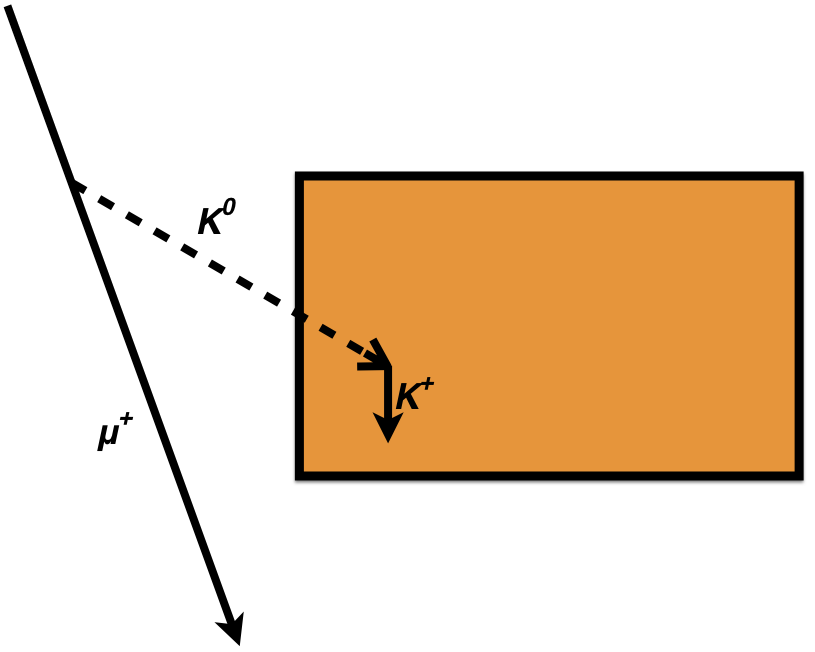
\includegraphics[width=0.5\textwidth]{KaonNDKInteraction}
  \caption[How the interaction of a cosmic muon can mimic a nucleon decay signature]
          {How the interaction of a cosmic muon can mimic a nucleon decay signature, by producing a $K^{0}_{L}$ which interacts far from the detector wall, producing an isolated kaon.}
  \label{fig:K0LongBackground}
\end{figure}

